\chapter{Membangun Model Prediksi}

Untuk pratikum saati ini menggunakan buku \textit{Python Artificial Intelligence Projects for Beginners}\cite{eckroth2018python}. Dengan praktek menggunakan python 3 dan editor anaconda dan library python scikit-learn.
Dataset ada di https://github.com/PacktPublishing/Python-Artificial-Intelligence-Projects-for-Beginners .
Tujuan pembelajaran pada pertemuan pertama antara lain:
\begin{enumerate}
\item
Mengerti implementasi klasifikasi
\item
Memahami data set, training dan testing data
\item
Memahami Decission tree.
\item
Memahami information gain dan entropi.
\end{enumerate}
Tugas dengan cara dikumpulkan dengan pull request ke github dengan menggunakan latex pada repo yang dibuat oleh asisten riset. Kode program menggunakan input listing ditaruh di folder src ekstensi .py dan dipanggil ke latex dengan input listings. Tulisan dan kode tidak boleh plagiat, menggunakan bahasa indonesia yang sesuai dengan gaya bahasa buku teks.

\section{Teori}
Praktek teori penunjang yang dikerjakan(nilai 5 per nomor, untuk hari pertama) :
\begin{enumerate}
\item
Jelaskan apa itu binary classification dilengkapi ilustrasi gambar sendiri
\begin{itemize}
 \newpage 
\item Binary Classification merupakan bentuk klasifikasi untuk proses memprediksi variable kategori dimana output dibatasi untuk kedua kelas.
\begin{figure}[h]
    \centering
    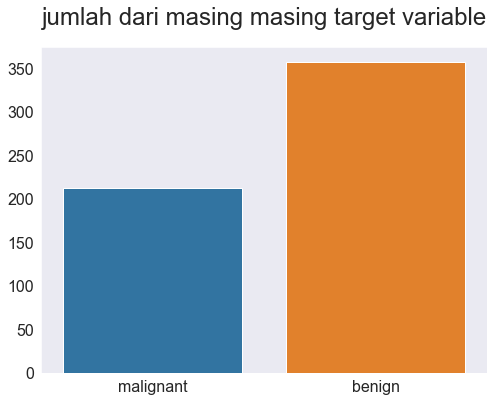
\includegraphics[scale=0.5]{figures/chapter 2/1.png}
    \caption{Binary Classification using dataset breast cancer}
    \label{fig:mesh1}
\end{figure}
\end{itemize}
\newpage \item
Jelaskan apa itu supervised learning dan unsupervised learning dan clustering dengan ilustrasi gambar sendiri.
\begin{itemize}
\item supervised learning merupakan Machine Learning model yang mempelajari data dengan label atau target dimana evaluasi model tersebut akan berdasarkan
target. contoh: pengenalan jenis bunga berdasarkan ukuran kelopak
dan warna kelopak. seperti pada Figure 2.2 merupakan hasil predict dan ciri dari sample dataset iris yang didapatkan dari algoritma SVC untuk memprediksi target dari suatu objek berdasarkan beberapa ciri seperti sepal length, sepal width, petal width dan sepal length, akan diprediksi menjadi salah satu dari beberapa target name seperti setosa, versicolor dan virginica.
\begin{figure}[h]
    \centering
    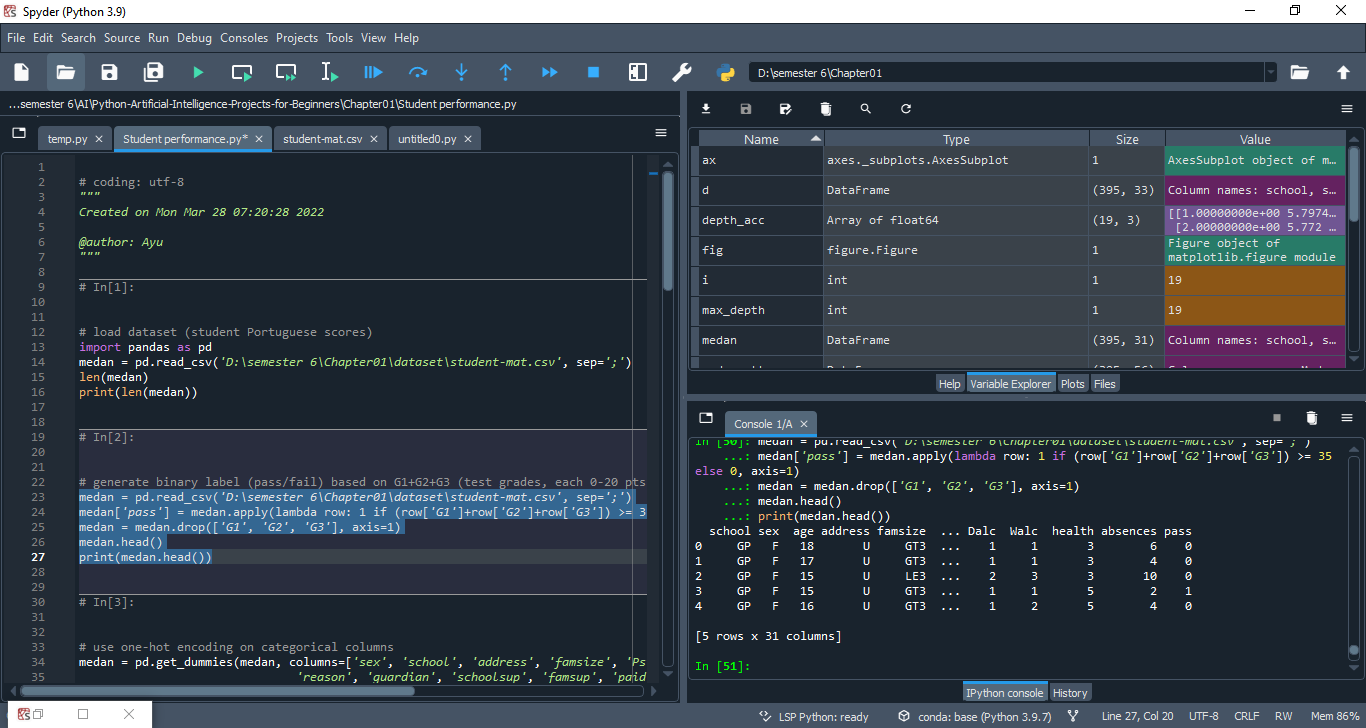
\includegraphics[scale=0.6]{figures/chapter 2/2.png}
    \caption{Contoh Hasil dari predict dari supervised learning menggunakan SVC}
    \label{fig:mesh1}
\end{figure}
\begin{figure}[h]
    \centering
    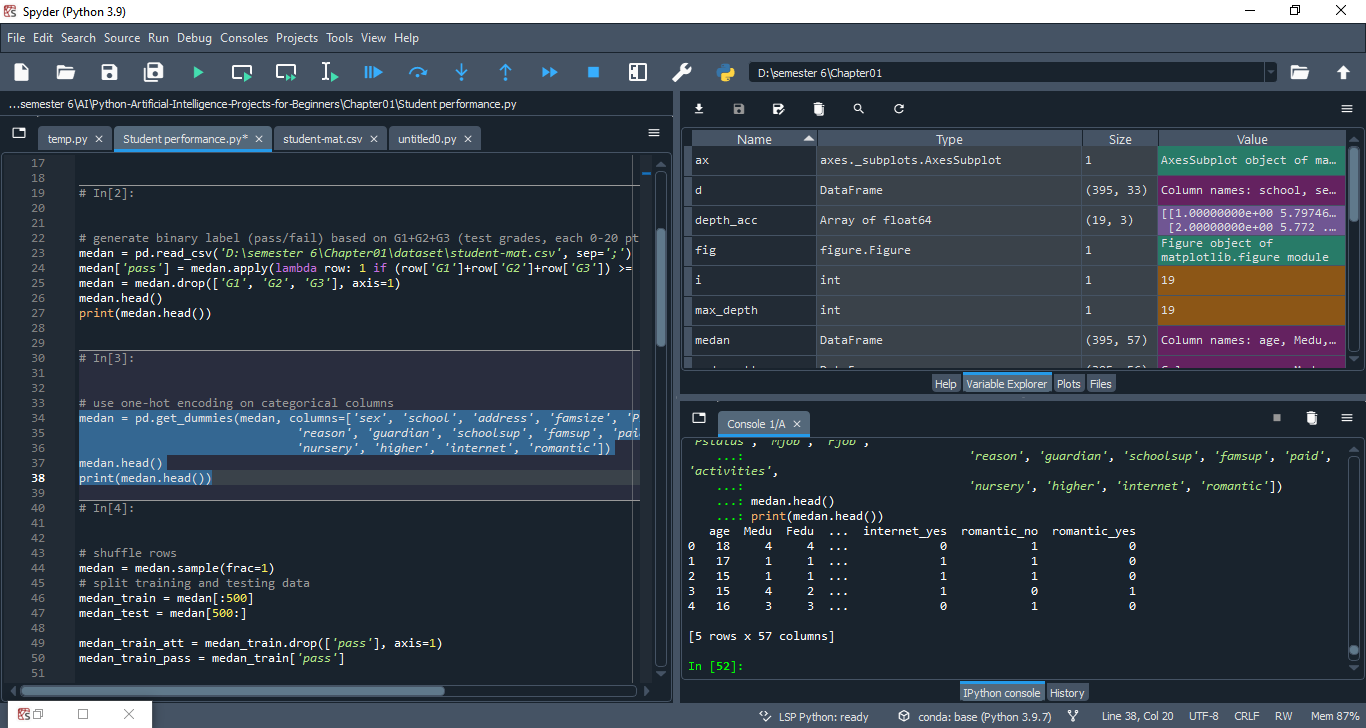
\includegraphics[scale=0.6]{figures/chapter 2/3.png}
    \caption{Source Code fitting dan predict menggunakan dataset iris pada model SVC}
    \label{fig:mesh1}
\end{figure}
\newpage
\item Unsupervised learning adalah salah satu tipe algoritma machine learning yang digunakan untuk menarik kesimpulan dari dataset. Metode ini hanya akan mempelajari suatu data berdasarkan kedekatannya saja atau yang biasa disebut dengan clustering. Metode unsupervised learning yang paling umum adalah analisis cluster, yang digunakan pada analisa data untuk mencari pola-pola tersembunyi atau pengelompokan dalam data.
\begin{figure}[h]
    \centering
    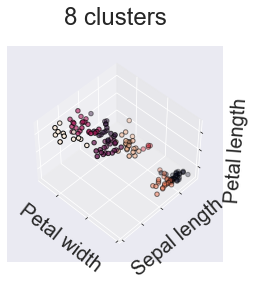
\includegraphics[scale=0.4]{figures/chapter 2/4.png}
    \caption{Binary Classification using dataset breast cancer}
    \label{fig:mesh1}
\end{figure}
\begin{figure}[h]
    \centering
    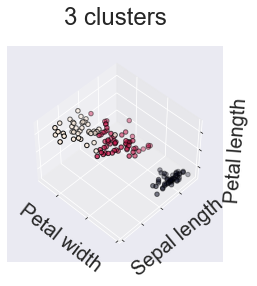
\includegraphics[scale=0.4]{figures/chapter 2/5.png}
    \caption{Binary Classification using dataset breast cancer}
    \label{fig:mesh1}
\end{figure}
\begin{figure}[h]
    \centering
    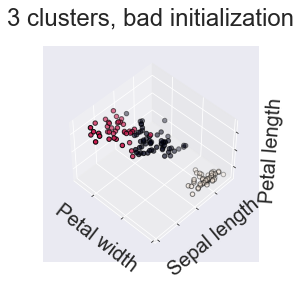
\includegraphics[scale=0.4]{figures/chapter 2/6.png}
    \caption{Binary Classification using dataset breast cancer}
    \label{fig:mesh1}
\end{figure}
\end{itemize}
\item
Jelaskan apa itu evaluasi dan akurasi dari buku dan disertai ilustrasi contoh dengan gambar sendiri
	\begin{itemize}
		\item akurasi dapat didefinisikan sebagai pendekatan pengukuran berdasarkan standar atau nilai sebenarnya yaitu, sistem navigasi yang sangat akurat akan memeberikan nilai pengukuran yang sangat kuat dengan nilai standar
		\item evaluasi dapat didefinisikan sebagai bagaimana mengukur seberapa baik nilai performa dari suatu model.
	\end{itemize}
\item
Jelaskan bagaimana cara membuat dan membaca confusion matrix, buat confusion matrix buatan sendiri.
	\begin{itemize}
		\item akurasi dapat didefinisikan sebagai pendekatan pengukuran berdasarkan standar atau nilai sebenarnya yaitu, sistem navigasi yang sangat akurat akan memeberikan nilai pengukuran yang sangat kuat dengan nilai standar
		\item evaluasi dapat didefinisikan sebagai bagaimana mengukur seberapa baik nilai performa dari suatu model.
	\end{itemize}
\item
Jelaskan bagaimana K-fold cross validation bekerja dengan gambar ilustrasi contoh buatan sendiri.
\item
Jelaskan apa itu decision tree dengan gambar ilustrasi contoh buatan sendiri.
\item
Jelaskan apa itu information gain dan entropi dengan gambar ilustrasi buatan sendiri.
\end{enumerate}

\section{scikit-learn}
Dataset ambil di https://github.com/PacktPublishing/Python-Artificial-Intelligence-Projects-for-Beginners folder Chapter01.
Tugas anda adalah, dataset ganti menggunakan \textbf{student-mat.csv} dan mengganti semua nama variabel dari kode di bawah ini dengan nama-nama makanan (NPM mod 3=0), kota (NPM mod 3=1), buah (NPM mod 3=2), . Jalankan satu per satu kode tersebut di spyder dengan menggunakan textit{Run current cell}. Kemudian Jelaskan dengan menggunakan bahasa yang mudah dimengerti dan bebas plagiat dan wajib skrinsut dari komputer sendiri masing masing nomor di bawah ini(nilai 5 masing masing pada hari kedua).

\begin{enumerate}

\item
\begin{verbatim}
	# load dataset (student mat pakenya)
	import pandas as pd
	d = pd.read_csv('student-mat.csv', sep=';')
	len(d)
\end{verbatim}
\begin{figure}[h]
    \centering
    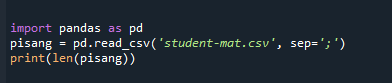
\includegraphics[scale=0.6]{figures/chapter 2/sklearn/1.png}
    \caption{Source Code Task 1}
    \label{fig:mesh1}
\end{figure}
\begin{figure}[h]
    \centering
    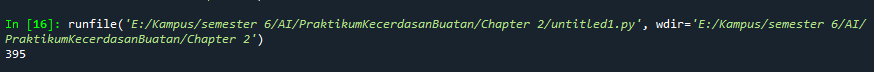
\includegraphics[scale=0.6]{figures/chapter 2/sklearn/2.png}
    \caption{Output Task 1}
    \label{fig:mesh1}
\end{figure}
\item
\begin{verbatim}
	# generate binary label (pass/fail) based on G1+G2+G3 
	# (test grades, each 0-20 pts); threshold for passing is sum>=30
	d['pass'] = d.apply(lambda row: 1 if (row['G1']+row['G2']+row['G3']) 
											>= 35 else 0, axis=1)
	d = d.drop(['G1', 'G2', 'G3'], axis=1)
	d.head()
\end{verbatim}
\begin{figure}[h]
    \centering
    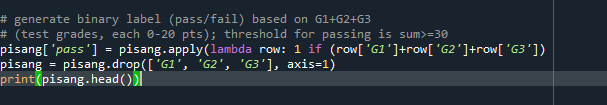
\includegraphics[scale=0.6]{figures/chapter 2/sklearn/3.png}
    \caption{Source Code Task 2}
    \label{fig:mesh1}
\end{figure}
\begin{figure}[h]
    \centering
    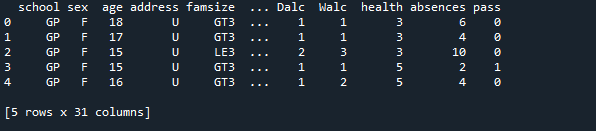
\includegraphics[scale=0.6]{figures/chapter 2/sklearn/4.png}
    \caption{Output Task 2}
    \label{fig:mesh1}
\end{figure}
\item
\begin{verbatim}
	# use one-hot encoding on categorical columns
	d = pd.get_dummies(d, columns=['sex', 'school', 'address', 
									'famsize', 
									'Pstatus', 'Mjob', 'Fjob', 
	                               'reason', 'guardian', 'schoolsup', 
								   'famsup', 'paid', 'activities',
	                               'nursery', 'higher', 'internet', 
									'romantic'])
	d.head()
\end{verbatim}
\newpage
\begin{figure}[h]
    \centering
    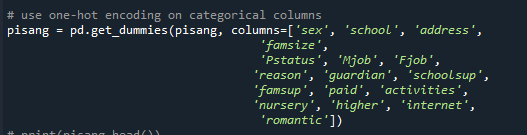
\includegraphics[scale=0.6]{figures/chapter 2/sklearn/5.png}
    \caption{Source Code Task 3}
    \label{fig:mesh1}
\end{figure}
\begin{figure}[h]
    \centering
    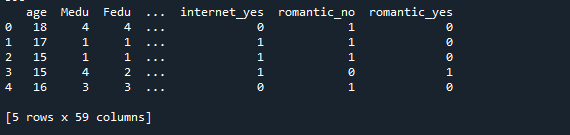
\includegraphics[scale=0.6]{figures/chapter 2/sklearn/6.png}
    \caption{Output Task 3}
    \label{fig:mesh1}
\end{figure}
\newpage
\item
\begin{verbatim}
	# shuffle rows
	d = d.sample(frac=1)
	# split training and testing data
	d_train = d[:500]
	d_test = d[500:]

	d_train_att = d_train.drop(['pass'], axis=1)
	d_train_pass = d_train['pass']

	d_test_att = d_test.drop(['pass'], axis=1)
	d_test_pass = d_test['pass']

	d_att = d.drop(['pass'], axis=1)
	d_pass = d['pass']

	# number of passing students in whole dataset:
	import numpy as np
	print("Passing: %d out of %d (%.2f%%)" % (np.sum(d_pass), len(d_pass), 
	       100*float(np.sum(d_pass)) / len(d_pass)))
\end{verbatim}
\begin{figure}[h]
    \centering
    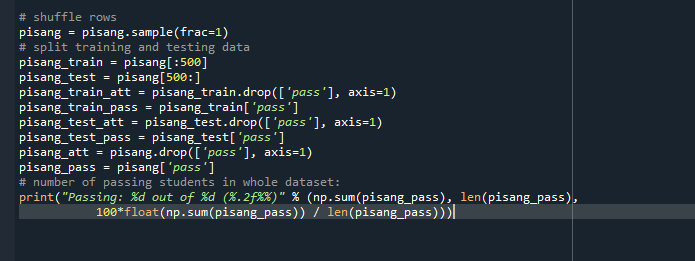
\includegraphics[scale=0.6]{figures/chapter 2/sklearn/7.png}
    \caption{Source Code Task 4}
    \label{fig:mesh1}
\end{figure}
\begin{figure}[h]
    \centering
    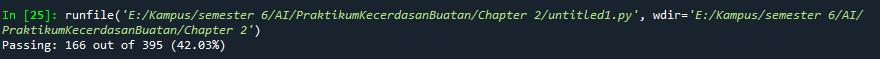
\includegraphics[scale=0.6]{figures/chapter 2/sklearn/8.png}
    \caption{Output Task 4}
    \label{fig:mesh1}
\end{figure}
\item 
\begin{verbatim}
	# fit a decision tree
	from sklearn import tree
	t = tree.DecisionTreeClassifier(criterion="entropy", max_depth=5)
	t = t.fit(d_train_att, d_train_pass)
\end{verbatim}
\begin{figure}[h]
    \centering
    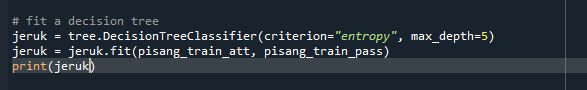
\includegraphics[scale=0.6]{figures/chapter 2/sklearn/9.png}
    \caption{Source Code Task 5}
    \label{fig:mesh1}
\end{figure}
\begin{figure}[h]
    \centering
    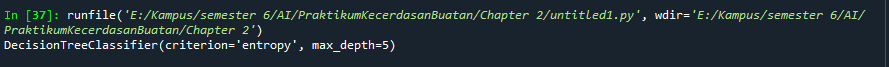
\includegraphics[scale=0.6]{figures/chapter 2/sklearn/10.png}
    \caption{Output Task 5}
    \label{fig:mesh1}
\end{figure}
\item
\begin{verbatim}
	# visualize tree
	import graphviz
	dot_data = tree.export_graphviz(t, out_file=None, label="all", 
									impurity=False, proportion=True,
	                                feature_names=list(d_train_att), 
									class_names=["fail", "pass"], 
	                                filled=True, rounded=True)
	graph = graphviz.Source(dot_data)
	graph
\end{verbatim}
\begin{figure}[h]
    \centering
    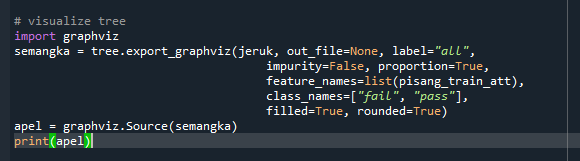
\includegraphics[scale=1]{figures/chapter 2/sklearn/11.png}
    \caption{Source Code Task 6}
    \label{fig:mesh1}
\end{figure}
\begin{figure}[h]
    \centering
    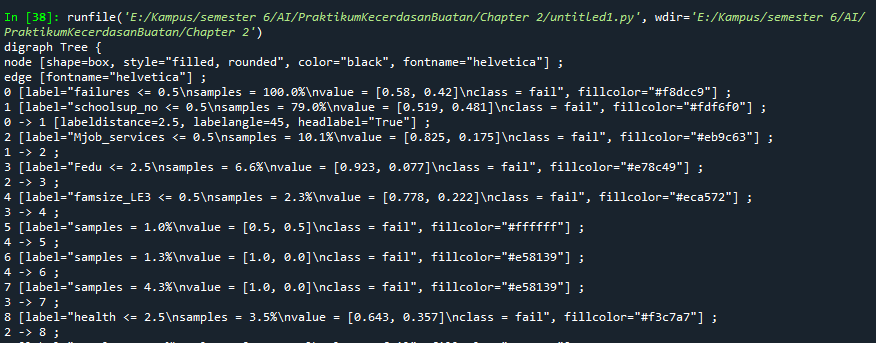
\includegraphics[scale=0.6]{figures/chapter 2/sklearn/12.png}
    \caption{Output Task 6}
    \label{fig:mesh1}
\end{figure}
\newpage \item
\begin{verbatim}
	# save tree
	tree.export_graphviz(t, out_file="student-performance.dot", 
						 label="all", impurity=False, 
						 proportion=True,
	                     feature_names=list(d_train_att), 
	                     class_names=["fail", "pass"], 
	                     filled=True, rounded=True)
\end{verbatim}
\begin{figure}[h]
    \centering
    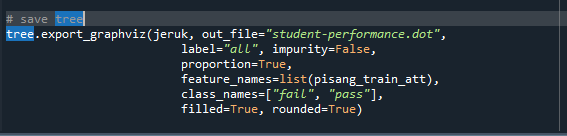
\includegraphics[scale=0.8]{figures/chapter 2/sklearn/13.png}
    \caption{Source Code Task 7}
    \label{fig:mesh1}
\end{figure}
\begin{figure}[h]
    \centering
    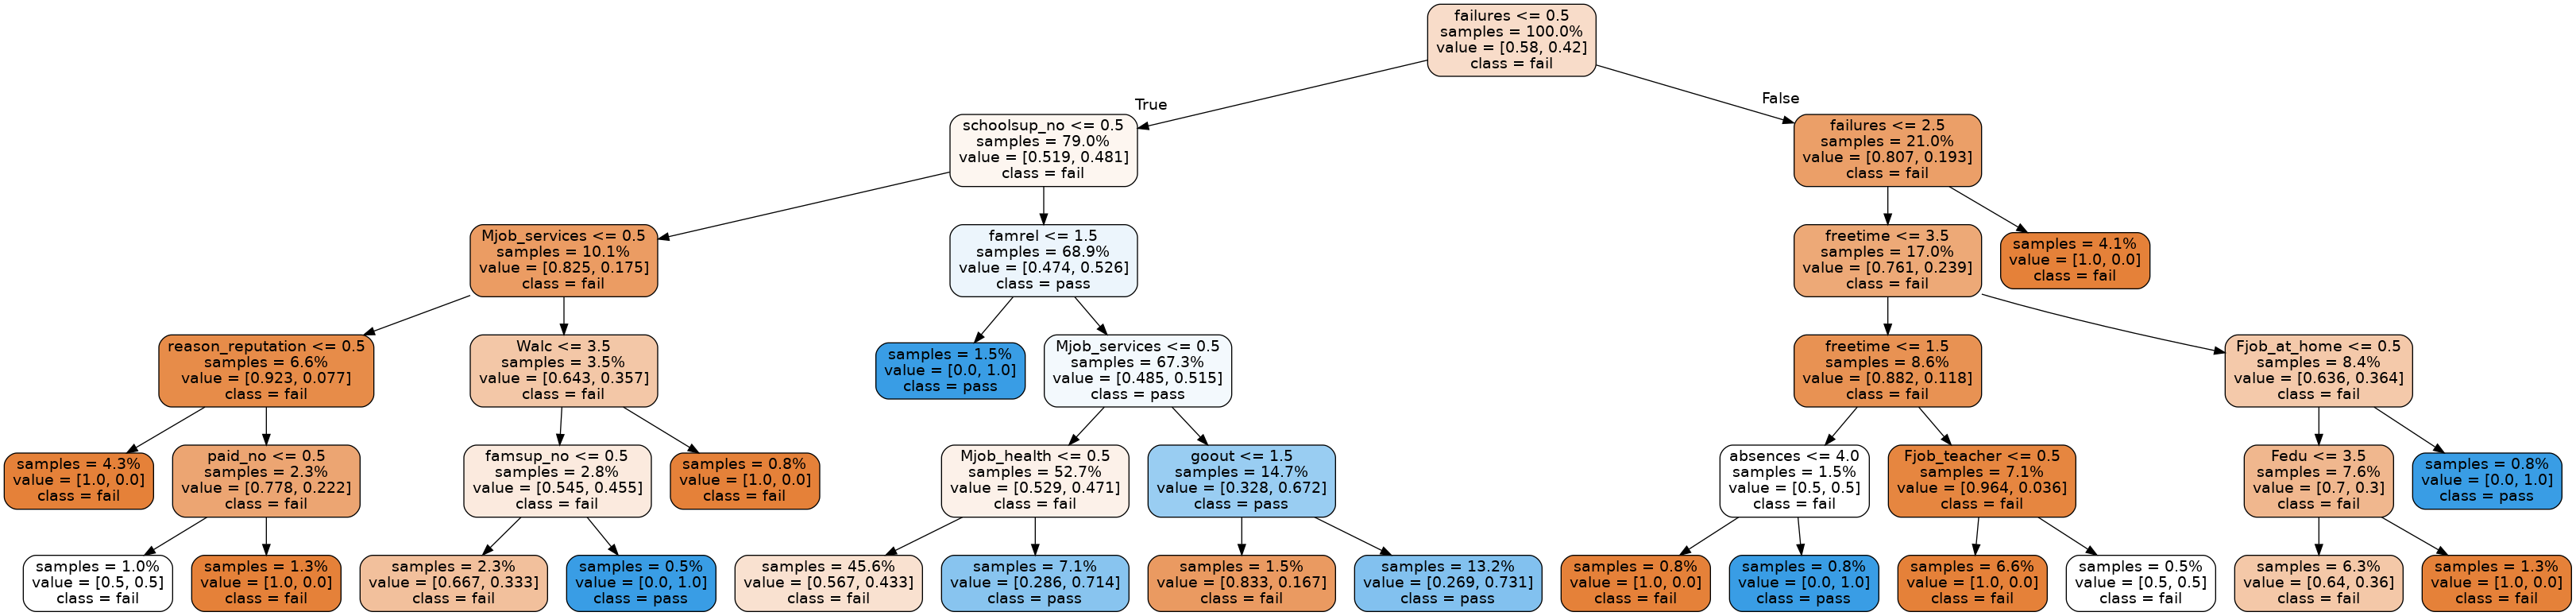
\includegraphics[scale=0.15]{figures/chapter 2/sklearn/14.png}
    \caption{Output Task 7}
    \label{fig:mesh1}
\end{figure}
\newpage
\item
\begin{verbatim}
	t.score(d_test_att, d_test_pass)
\end{verbatim}
\begin{figure}[h]
    \centering
    
\includegraphics[scale=1]{figures/chapter 2/sklearn/15.png}
    \caption{Source Code Task 8}
    \label{fig:mesh1}
\end{figure}
\begin{figure}[h]
    \centering
    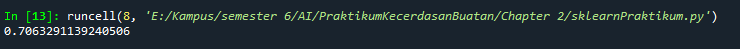
\includegraphics[scale=0.7]{figures/chapter 2/sklearn/16.png}
    \caption{Output Task 8}
    \label{fig:mesh1}
\end{figure}
\item
\begin{verbatim}
	from sklearn.model_selection import cross_val_score
	scores = cross_val_score(t, d_att, d_pass, cv=5)
	# show average score and +/- two standard deviations away 
	#(covering 95% of scores)
	print("Accuracy: %0.2f (+/- %0.2f)" % (scores.mean(), scores.std() * 2))
\end{verbatim}
\begin{figure}[h]
    \centering
    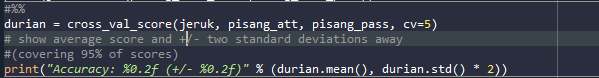
\includegraphics[scale=0.8]{figures/chapter 2/sklearn/17.png}
    \caption{Source Code Task 9}
    \label{fig:mesh1}
\end{figure}
\begin{figure}[h]
    \centering
    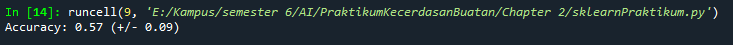
\includegraphics[scale=0.8]{figures/chapter 2/sklearn/18.png}
    \caption{Output Task 9}
    \label{fig:mesh1}
\end{figure}
\newpage
\item 
\begin{verbatim}
	for max_depth in range(1, 20):
	    t = tree.DecisionTreeClassifier(criterion="entropy", 
			max_depth=max_depth)
	    scores = cross_val_score(t, d_att, d_pass, cv=5)
	    print("Max depth: %d, Accuracy: %0.2f (+/- %0.2f)" % 
				(max_depth, scores.mean(), scores.std() * 2)
			 )
\end{verbatim}
\begin{figure}[h]
    \centering
    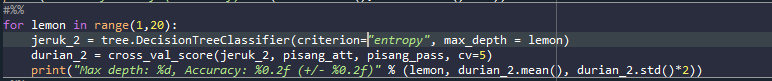
\includegraphics[scale=0.6]{figures/chapter 2/sklearn/19.png}
    \caption{Source Code Task 10}
    \label{fig:mesh1}
\end{figure}
\begin{figure}[h]
    \centering
    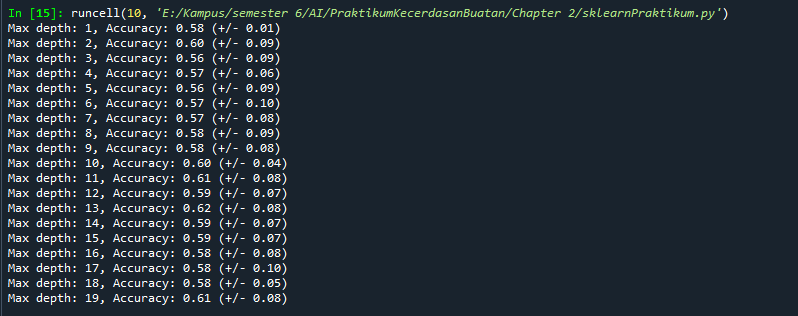
\includegraphics[scale=0.6]{figures/chapter 2/sklearn/20.png}
    \caption{Output Task 10}
    \label{fig:mesh1}
\end{figure}
\item
\begin{verbatim}
	depth_acc = np.empty((19,3), float)
	i = 0
	for max_depth in range(1, 20):
	    t = tree.DecisionTreeClassifier(criterion="entropy", 
			max_depth=max_depth)
	    scores = cross_val_score(t, d_att, d_pass, cv=5)
	    depth_acc[i,0] = max_depth
	    depth_acc[i,1] = scores.mean()
	    depth_acc[i,2] = scores.std() * 2
	    i += 1

	depth_acc
\end{verbatim}
\begin{figure}[h]
    \centering
    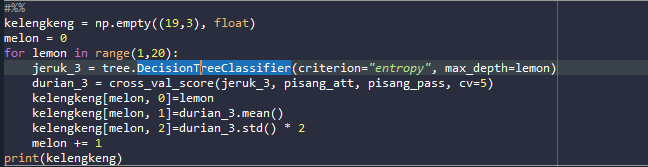
\includegraphics[scale=0.6]{figures/chapter 2/sklearn/21.png}
    \caption{Source Code Task 11}
    \label{fig:mesh1}
\end{figure}
\begin{figure}[h]
    \centering
    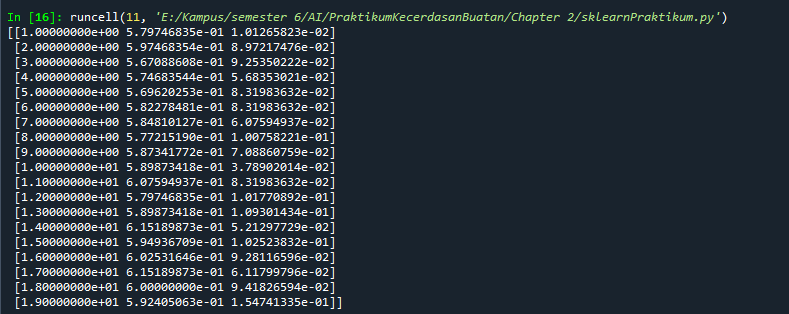
\includegraphics[scale=0.6]{figures/chapter 2/sklearn/22.png}
    \caption{Output Task 11}
    \label{fig:mesh1}
\end{figure}
\newpage
\item 
\begin{verbatim}
	import matplotlib.pyplot as plt
	fig, ax = plt.subplots()
	ax.errorbar(depth_acc[:,0], depth_acc[:,1], yerr=depth_acc[:,2])
	plt.show()
\end{verbatim}
\begin{figure}[h]
    \centering
    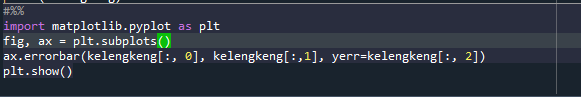
\includegraphics[scale=0.6]{figures/chapter 2/sklearn/23.png}
    \caption{Source Code Task 12}
    \label{fig:mesh1}
\end{figure}
\begin{figure}[h]
    \centering
    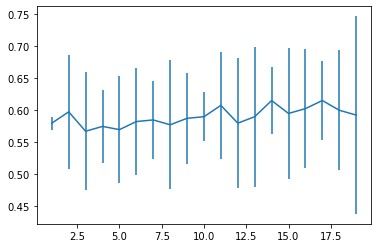
\includegraphics[scale=0.6]{figures/chapter 2/sklearn/24.png}
    \caption{Output Task 12}
    \label{fig:mesh1}
\end{figure}

\end{enumerate}


\section{Penanganan Error}
Dari percobaan yang dilakukan di atas, error yang kita dapatkan di dokumentasikan dan di selesaikan(nilai 5 hari kedua):

\begin{enumerate}
	\item
skrinsut error
	\item
Tuliskan kode eror dan jenis errornya
	\item
Solusi pemecahan masalah error tersebut

\end{enumerate}

